\let\negmedspace\undefined
\let\negthickspace\undefined
\documentclass[journal,12pt,twocolumn]{IEEEtran}

\usepackage{csquotes}
\usepackage{comment}
\usepackage{enumerate}
\usepackage{amsmath,amssymb,amsthm}
\usepackage{graphicx}
\let\vec\mathbf
\newcommand{\myvec}[1]{\ensuremath{\begin{pmatrix}#1\end{pmatrix}}}
\providecommand{\brak}[1]{\ensuremath{\left(#1\right)}}
\providecommand{\pr}[1]{\ensuremath{\Pr\left(#1\right)}}
 \title{Assignment 3}
     \author{AKKASANI YAGNESH REDDY \\
     cs21btech11003 \\}
     
     \begin{document}
     \maketitle
     \textbf{Question:}We have four boxes. Box $1$ contains $2000$ components of which $5\%$ are defective.Box $2$ contains $500$ components of which $40\%$ are defective. Boxes $3$ and $4$ contain 1000 each with $10\%$ defective. We select at random one of the boxes and we remove at random a single component.\\
     a) What is the probability that the selected component is defective?\\
     b)We examine the selected component and we find it defective. On the basis of this evidence, we want to determine the probability that it came from box 2.
     
     
     \textbf{Solution:}\\
Let the random variable $Y$ take values,\\
     \begin{table}[h!]
    \centering
    \begin{tabular}{|c|c|c|} \hline
    \textbf{Variable} & \textbf{Value} & \textbf{description} \\ \hline
         $Y$ & $0$ & If the item is found to defective \\ \hline
         $Y$ & $1$ & If the item is found to be non-defective.\\ \hline
     \end{tabular}
     \end{table}
     
Let the random variable X take values,\\
 \begin{table}[h!]
    \centering
    \begin{tabular}{|c|c|c|} \hline
    \textbf{Variable} & \textbf{Value} & \textbf{description} \\ \hline
    $X$ & $0$ & If the item is from box 1 \\ \hline
        $X$ & $1$ & If the item is from box 2 \\ \hline
        $X$ & $2$ & If the item is from box 3 \\ \hline
        $X$ & $2$ & If the item is from box 4 \\ \hline
    
    \end{tabular}
    \end{table}
    
    a) By total probability theorem;
    
    \begin{multline}
    \begin{split}
    \pr{Y=0}=\pr{X=0}*\pr{Y=0|X=0}\\+\pr{X=1}*\pr{Y=0|X=1}\\+
        \pr{X=2}*\pr{Y=0|X=2}\\+\pr{X=3}*\pr{Y=0|X=3}
\end{split}
\end{multline}
\begin{align}
    \pr{Y=0} &=\frac{1}{4}(0.05+0.4+0.1+0.1)\\
    \Rightarrow\pr{Y=0} &=0.1624
\end{align}    
  
    b) By bayes theorem;
    \begin{align}
           \pr{X=1|Y=0}&=\frac{\pr{X=1}*\pr{Y=0|X=1}}{\pr{Y=0}}\\
           \pr{X=1|Y=0}&=\frac{0.4*0.25}{0.1625}\\
           \pr{X=1|Y=0}&=0.6153
    \end{align}
    \newpage
      \begin{figure}[h!]
        \centering
        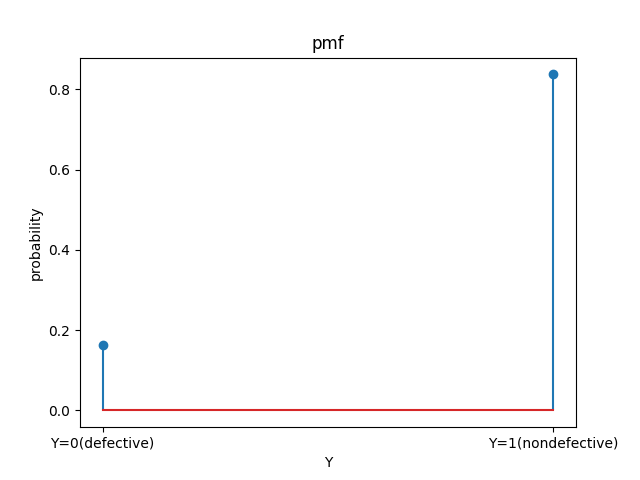
\includegraphics[scale=0.65]{Figure_1.png}
        \caption{pmf}
        \label{fig:my_label}
    \end{figure}
      \begin{figure}[h]
          \centering
          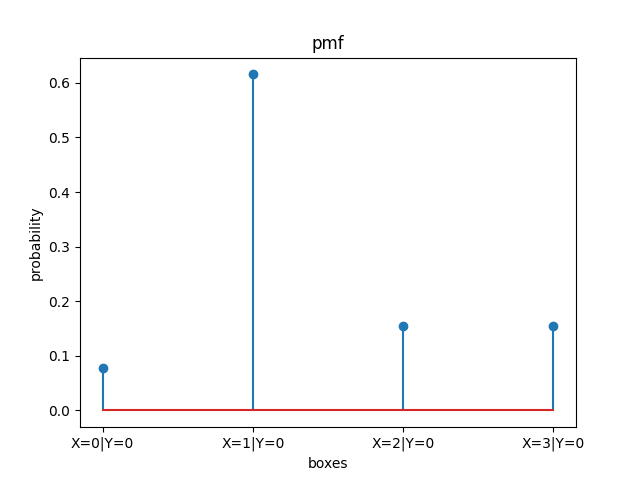
\includegraphics[scale=0.65]{Figure_2.png}
          \caption{pmf}
          \label{fig:my_label}
      \end{figure}
    
    
   \end{document}
     
